\documentclass{beamer}\usepackage[]{graphicx}\usepackage[]{color}
%% maxwidth is the original width if it is less than linewidth
%% otherwise use linewidth (to make sure the graphics do not exceed the margin)
\makeatletter
\def\maxwidth{ %
  \ifdim\Gin@nat@width>\linewidth
    \linewidth
  \else
    \Gin@nat@width
  \fi
}
\makeatother

\definecolor{fgcolor}{rgb}{0.345, 0.345, 0.345}
\newcommand{\hlnum}[1]{\textcolor[rgb]{0.686,0.059,0.569}{#1}}%
\newcommand{\hlstr}[1]{\textcolor[rgb]{0.192,0.494,0.8}{#1}}%
\newcommand{\hlcom}[1]{\textcolor[rgb]{0.678,0.584,0.686}{\textit{#1}}}%
\newcommand{\hlopt}[1]{\textcolor[rgb]{0,0,0}{#1}}%
\newcommand{\hlstd}[1]{\textcolor[rgb]{0.345,0.345,0.345}{#1}}%
\newcommand{\hlkwa}[1]{\textcolor[rgb]{0.161,0.373,0.58}{\textbf{#1}}}%
\newcommand{\hlkwb}[1]{\textcolor[rgb]{0.69,0.353,0.396}{#1}}%
\newcommand{\hlkwc}[1]{\textcolor[rgb]{0.333,0.667,0.333}{#1}}%
\newcommand{\hlkwd}[1]{\textcolor[rgb]{0.737,0.353,0.396}{\textbf{#1}}}%
\let\hlipl\hlkwb

\usepackage{framed}
\makeatletter
\newenvironment{kframe}{%
 \def\at@end@of@kframe{}%
 \ifinner\ifhmode%
  \def\at@end@of@kframe{\end{minipage}}%
  \begin{minipage}{\columnwidth}%
 \fi\fi%
 \def\FrameCommand##1{\hskip\@totalleftmargin \hskip-\fboxsep
 \colorbox{shadecolor}{##1}\hskip-\fboxsep
     % There is no \\@totalrightmargin, so:
     \hskip-\linewidth \hskip-\@totalleftmargin \hskip\columnwidth}%
 \MakeFramed {\advance\hsize-\width
   \@totalleftmargin\z@ \linewidth\hsize
   \@setminipage}}%
 {\par\unskip\endMakeFramed%
 \at@end@of@kframe}
\makeatother

\definecolor{shadecolor}{rgb}{.97, .97, .97}
\definecolor{messagecolor}{rgb}{0, 0, 0}
\definecolor{warningcolor}{rgb}{1, 0, 1}
\definecolor{errorcolor}{rgb}{1, 0, 0}
\newenvironment{knitrout}{}{} % an empty environment to be redefined in TeX

\usepackage{alltt}
\usepackage{../371g-slides}
\title{Introduction to predictive analytics}
\subtitle{Lecture 1}
\author{STA 371G}
\IfFileExists{upquote.sty}{\usepackage{upquote}}{}
\begin{document}



  \frame{\maketitle}

  % Show outline at beginning of each section
  \AtBeginSection[]{
    \begin{frame}<beamer>
      \tableofcontents[currentsection]
    \end{frame}
  }

  %%%%%%% Slides start here %%%%%%%

  \begin{darkframes}
    \begin{frame}{Course goals}
      \begin{itemize}
        \item Use regression and time series analysis to build predictive models
        \item Utilize simulations to forecast outputs based on uncertain inputs
        \item Given a new business situation, select an appropriate analysis, carry it out, and effectively communicate the results
        \item \alert{This is a practical course!}
      \end{itemize}
    \end{frame}

    % TODO: Update for instructor
    \begin{frame}{About the course staff}
      \begin{itemize}
        \item Instructor: \textbf{Brian Lukoff, Ph.D.}
          \begin{itemize}
            \item Office hours: M/W 11 AM-12 PM in CBA 3.440
            \item Contact: \texttt{brian.lukoff@utexas.edu} or 415-652-8853
          \end{itemize}
        \item TAs:
          \begin{itemize}
            \item Office hours: M 11:30 AM-1:30 PM, 2-4 PM, W 12-2 PM, Th 4-6 PM in CBA 4.304
            \item Help session: T 6-7 PM in the ModLab
          \end{itemize}

          \vspace{0.2in}
          \begin{center}
            \begin{tabular}{ccc}
              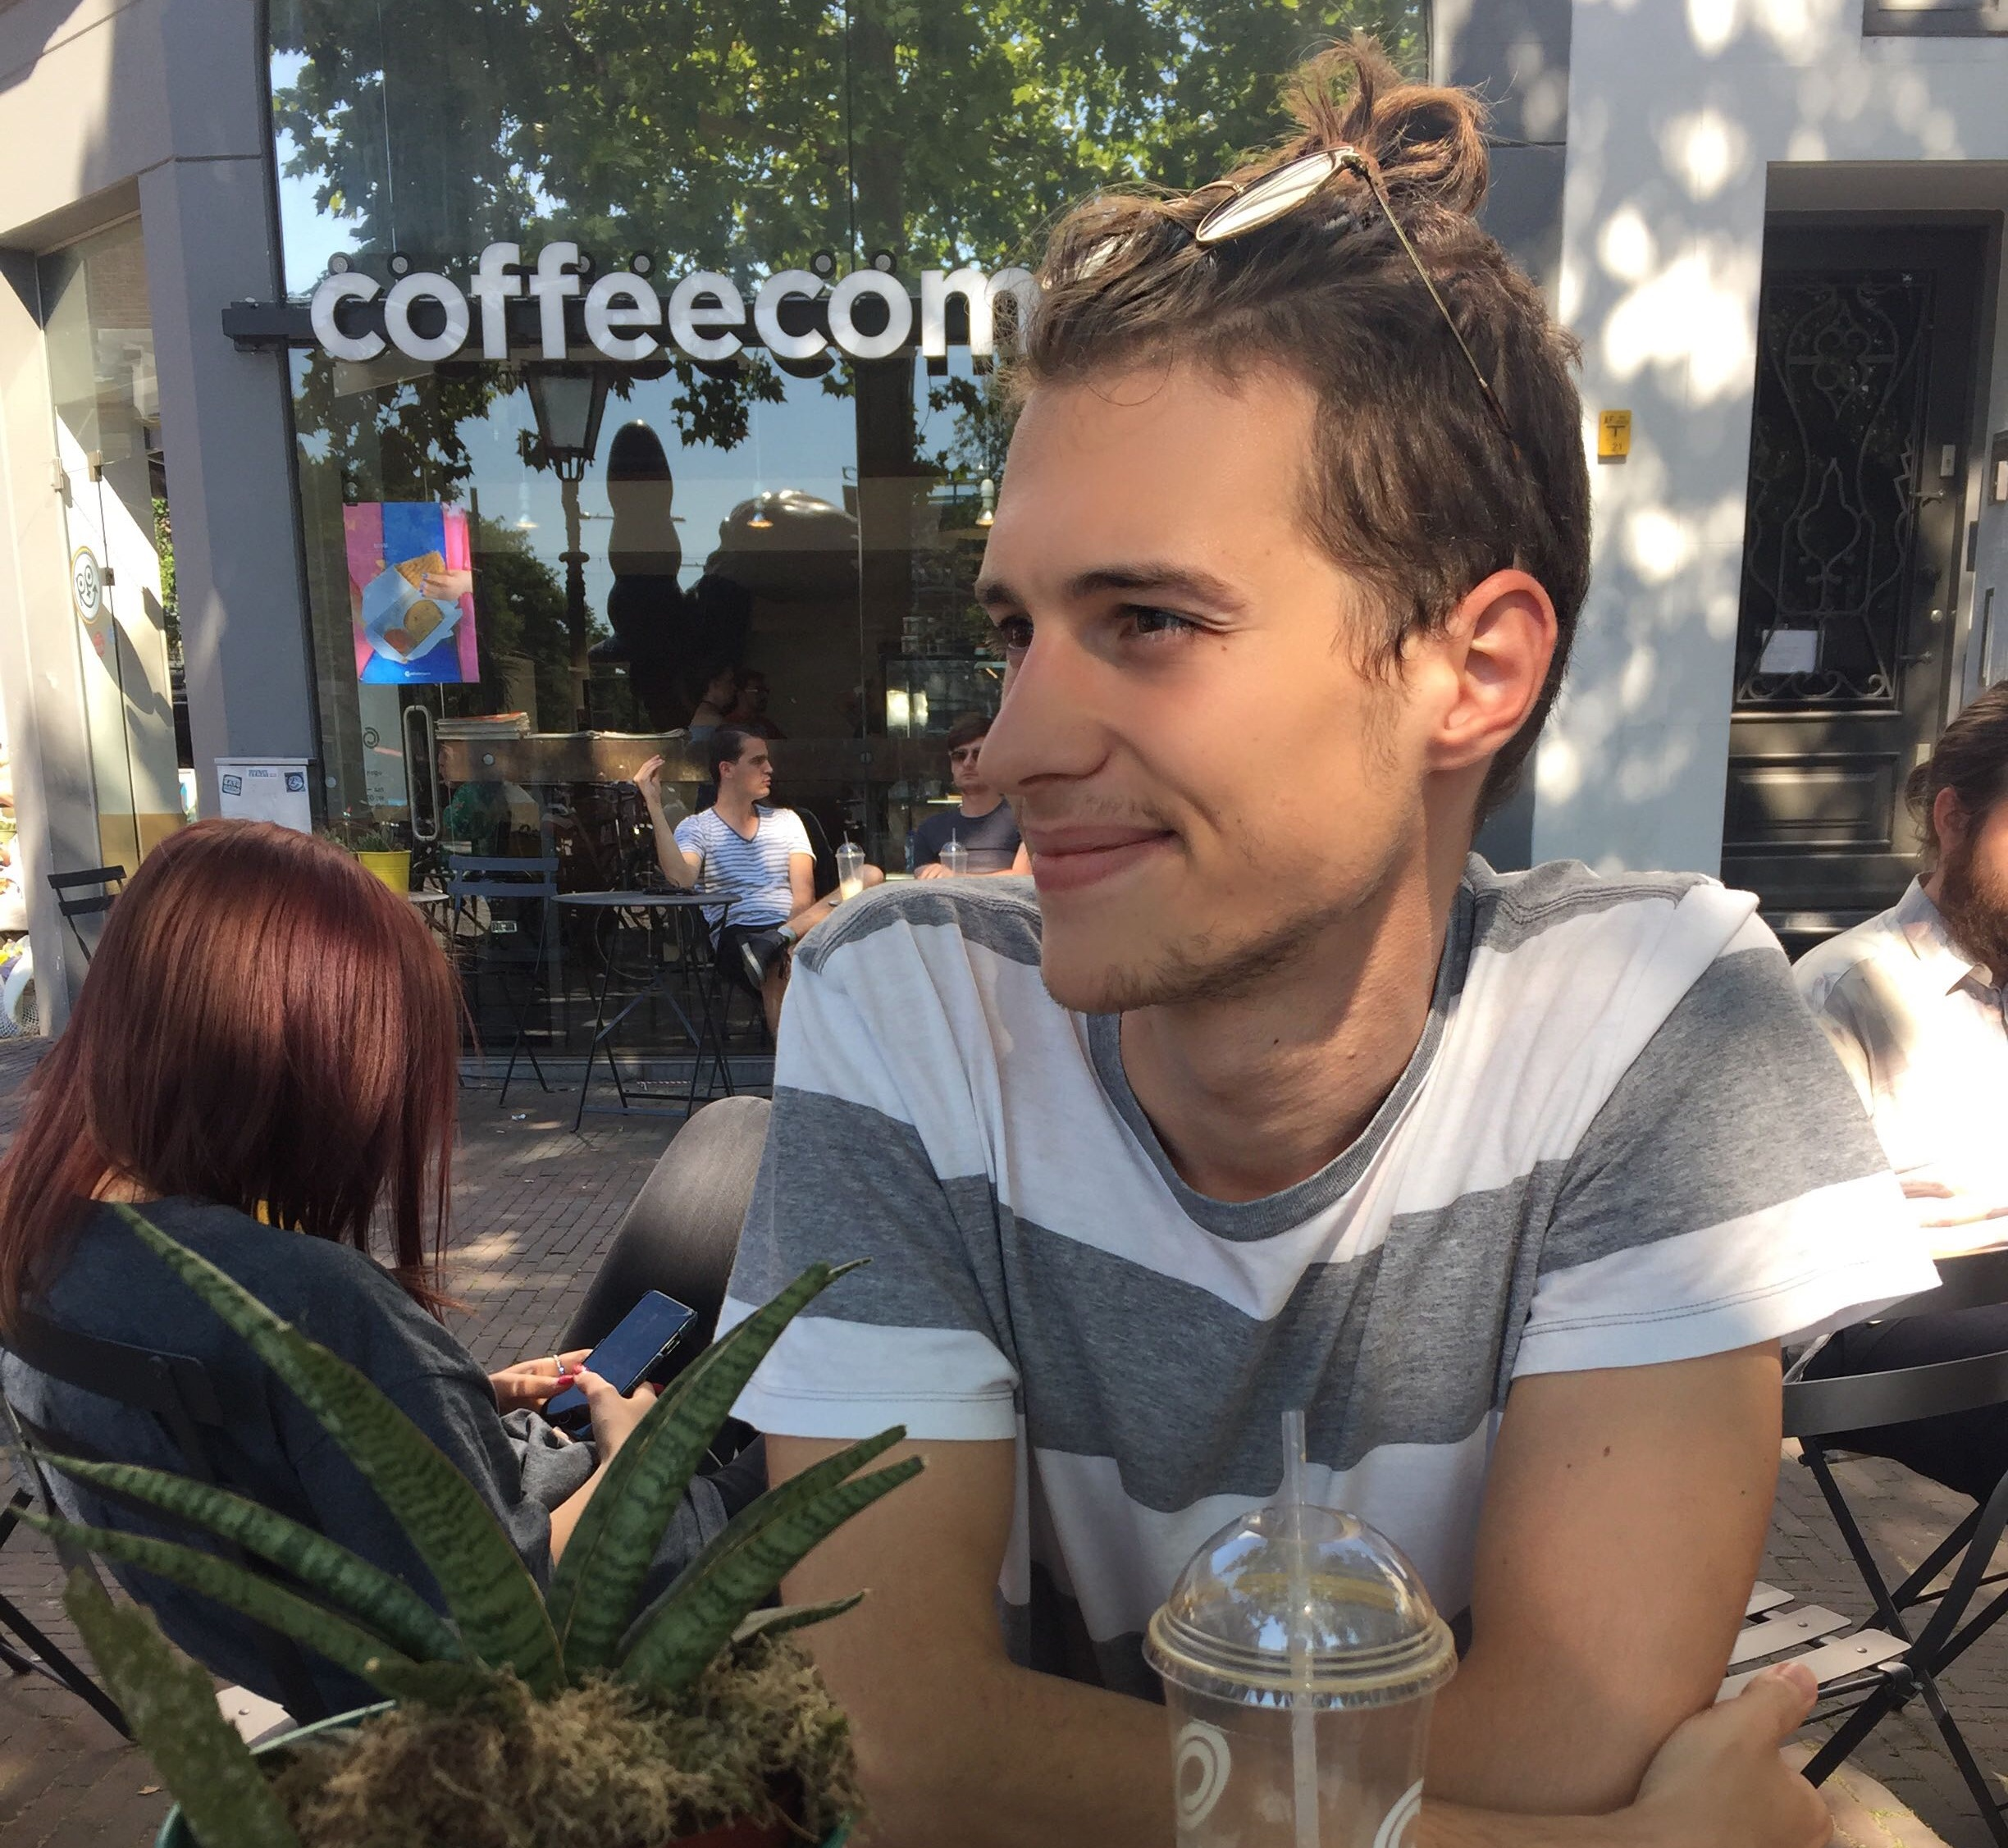
\includegraphics[width=1.1in]{vasko} &
              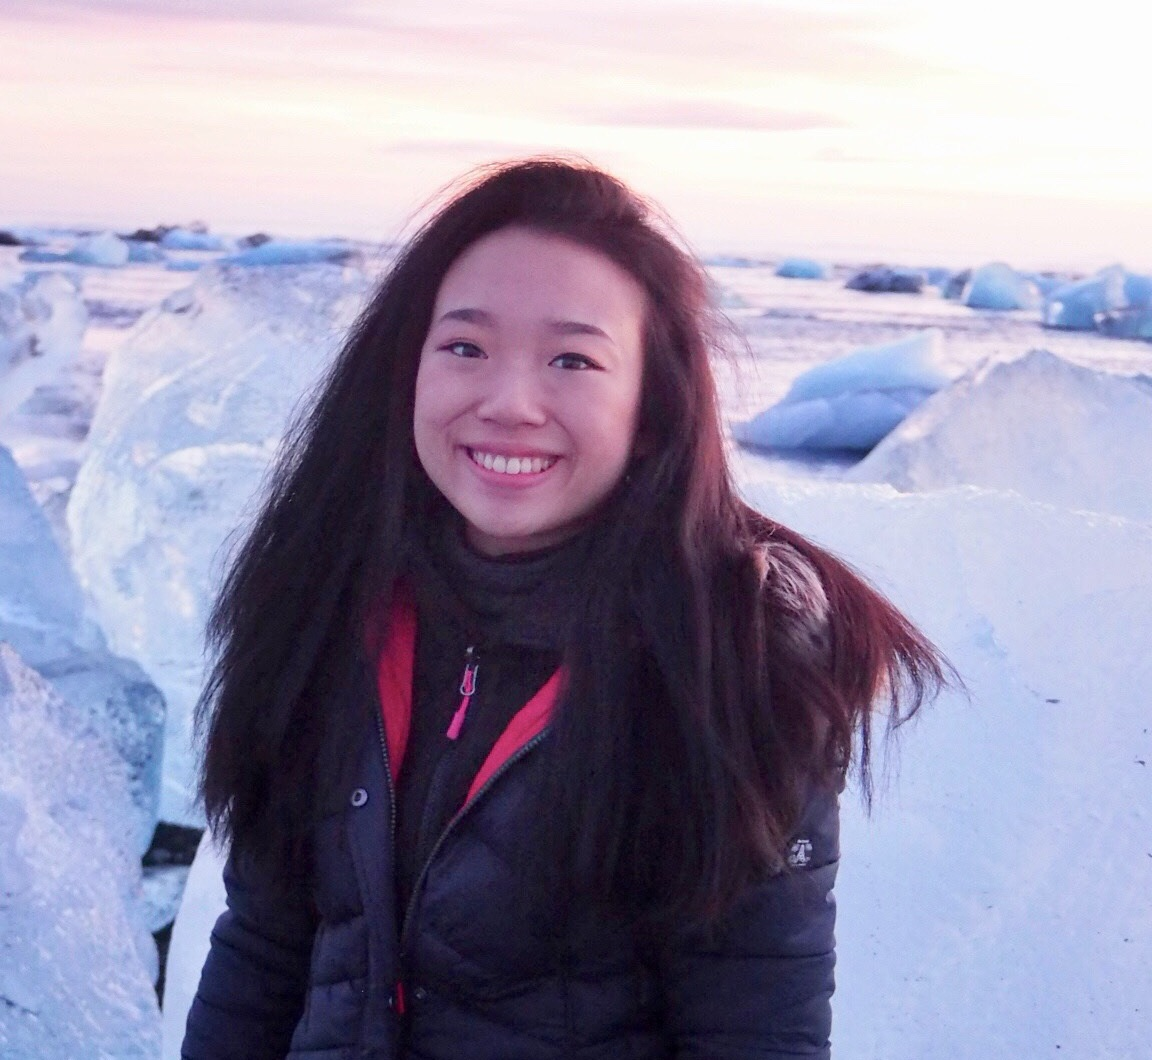
\includegraphics[width=1.1in]{nicole} &
              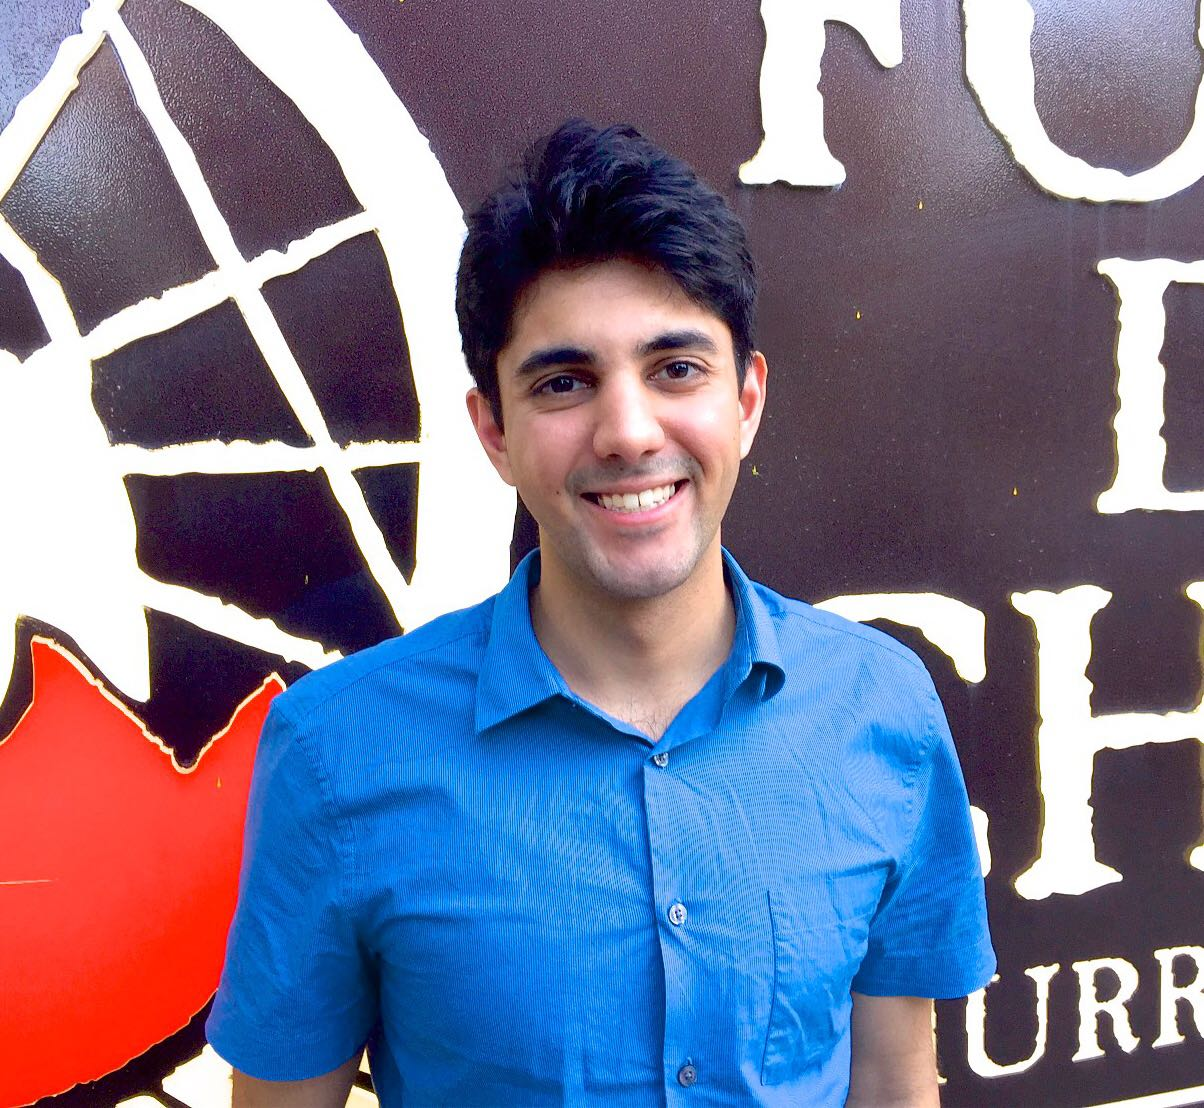
\includegraphics[width=1.1in]{zameer} \\
              Vasko Lalkov & Nicole Chia & Zameer Vaswani \\
            \end{tabular}
          \end{center}
      \end{itemize}
    \end{frame}

    % TODO: Update for instructor
    \begin{frame}{Who am I?}
      \begin{itemize}
        \item \textbf{Educator:} Teaching statistics at McCombs since 2014; previously taught at Harvard University and Boston University
        \item \textbf{Entrepreneur:} Currently co-founder and CEO of Perusall; formerly co-founder and CEO of Learning Catalytics (acquired by Pearson)
        \item \textbf{Engineer/statistician:} Software engineering/analytics background
      \end{itemize}
    \end{frame}

    \section{Find someone who...}

    \begin{frame}{}
      \begin{center}
        For each box on your bingo card, find someone who matches the description in the box. You must use a different person for each box.
        \vfill
        The winner will be crowned the STA 371G Bingo Champion$^{\text{TM}}$.
      \end{center}
    \end{frame}

    \section{Course logistics}

    \begin{frame}{Canvas}
      \begin{itemize}
        \item Access at \url{canvas.utexas.edu}
        \item This is your home base for the course
        \item Make sure you can log in and are enrolled in STA 371G in Canvas
      \end{itemize}
    \end{frame}

    \begin{frame}{Class participation}
      \begin{itemize}
        \item Understanding the concepts really only comes from practice
        \item We will use \alert{Learning Catalytics} so you can practice the concepts during class
        \item No cost to use this
        \item Graded on participation, not correctness; answer 75\% of the questions to get 100\% of the credit
        \item Bring a laptop to every class (check one out from the Media Center if needed)
        \item A note about devices in class
      \end{itemize}
    \end{frame}


    \begin{frame}{Homework}
      \begin{itemize}
        \item Why homework?
        \item 10 homework assignments during the semester
        \item We will use \alert{MyStatLab} for online homework; purchase and register through Canvas (you'll get a 2-week free trial)
      \end{itemize}
    \end{frame}


    \begin{frame}{Textbook}
      \begin{columns}[onlytextwidth]
        \column{.6\textwidth}
        \begin{itemize}
          \item Access the textbook as an eBook through MyStatLab OR buy a hardcover or looseleaf textbook (Sharpe, \emph{Business Statistics}, 4th ed) that includes a MyStatLab access code
          \item Reading ``quizzes'' are due by 7 PM; submit 2 questions for each reading about things that you found confusing/interesting
        \end{itemize}
        \column{.35\textwidth}
          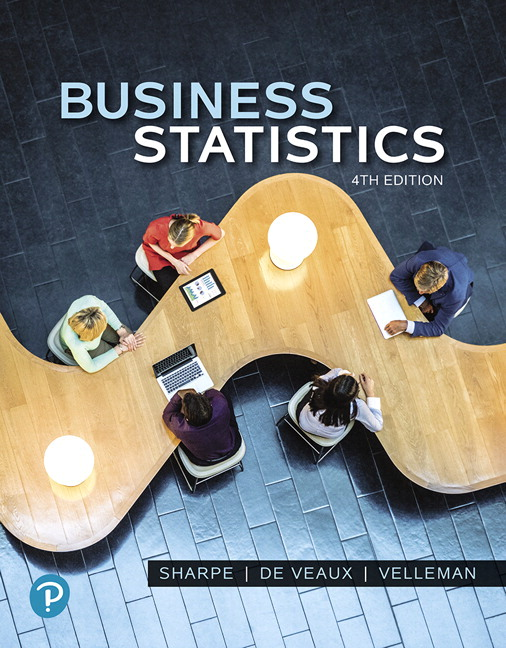
\includegraphics[width=1.5in]{textbook}
      \end{columns}
    \end{frame}

    \begin{frame}{Statistical computing}
      \begin{columns}[onlytextwidth]
        \column{.6\textwidth}
          \begin{itemize}
            \item We will use \alert{R} for statistical analysis throughout the course
            \item This is industrial-strength, state-of-the-art, and free software for statistical computing
            \item We will access R through \alert{RStudio}, a graphical interface for R
            \item Download R and RStudio at \url{rstudio.com}
          \end{itemize}
        \column{.3\textwidth}
          
\includegraphics[width=1in]{R}
      \end{columns}
    \end{frame}

    \begin{frame}{Exams}
      \begin{itemize}
        \item Two midterm exams and a cumulative final exam
        \item All are given during class time; you'll take the test on your laptop in this room
        \item You'll have access to R during every exam
        \item I will drop the lowest of your three exam scores (unless the final exam is your lowest grade)
      \end{itemize}
    \end{frame}

    \begin{frame}{Team project}
      \begin{itemize}
        \item You will pick a data set (or create one, e.g. through a survey) and apply regression techniques (we'll learn about this!) to build a predictive model
        \item Six deliverables throughout the semester:
        \begin{enumerate}
        \item Draft proposal
        \item Final proposal
        \item Review of related work
        \item Exploratory data analysis
        \item Write up results as a paper
        \item Presentation to class (during the finals period, on May 17)
        \end{enumerate}
      \end{itemize}
    \end{frame}

    \begin{frame}{Pretest}
      \begin{itemize}
        \item It is critical that you be up-to-speed on the prerequisite material covered in STA 309
        \item By January 31, complete a \alert{pretest} online to confirm your proficiency
        \item If you don't do well, expect to have to review some material on your own to avoid falling behind
      \end{itemize}
    \end{frame}

    \begin{frame}{Grading}
      \begin{center}
        \begin{tabular}{ll}
          Pretest             & \textbf{1\%}  \\
          Learning Catalytics & \textbf{5\%}  \\
          Reading quizzes     & \textbf{5\%}  \\
          Homework            & \textbf{14\%} \\
          Team project        & \textbf{15\%} \\
          Exams               & \textbf{60\%} \\
        \end{tabular}
      \end{center}
    \end{frame}

    \begin{frame}{PLUS (Peer-Led Undergraduate Studying)}
      \begin{columns}[onlytextwidth]
        \column{.4\textwidth}
          \begin{itemize}
            \item Weekly, student-run study groups
            \item You can apply to be a facilitator or just participate in any of the sessions
            \item Students who attend more PLUS sessions tend to get higher grades!
          \end{itemize}
        \column{.5\textwidth}
          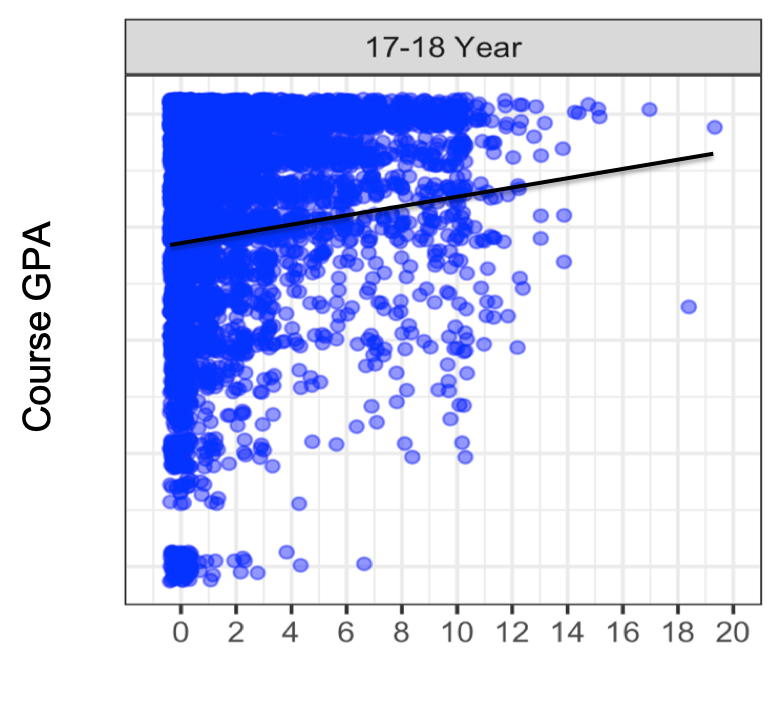
\includegraphics[width=2in]{plus}
      \end{columns}
    \end{frame}

    \begin{frame}{How to get an A in STA 371G}
      \begin{itemize}
        \item Work on more problems than are assigned in the homework; can find problems in the book and on MyStatLab
        \item Consider attending the optional R help sessions in the ModLab
        \item Consider attending the PLUS sessions
        \item Get help when you need it
          \begin{itemize}
            \item My office hours (after every class, until 12 PM)
            \item TA office hours (see syllabus for schedule)
            \item E-mail me to ask questions or set up a special appointment
          \end{itemize}
      \end{itemize}
    \end{frame}

    \section{Let's do some statistics, yo}

    \begin{frame}{Purpose of a model}
      \begin{itemize}
        \item \textbf{Make a prediction} about one variable based on the others
        \item \textbf{Understand the relationships} between the variables
      \end{itemize}
    \end{frame}

    \begin{frame}{Data analysis process}
      \begin{center}
        \tikzstyle{block} = [rectangle, draw, fill=darkgray,
            text width=8em, text centered, rounded corners, minimum height=2em]
        \tikzstyle{line} = [draw, -latex']

        \begin{tikzpicture}[node distance = 1.4cm, auto]
          \node [block] (define) {define problem};
          \node [block, below of=define] (explore) {explore the data};
          \node [block, below of=explore] (build) {build model};
          \node [block, below of=build] (evaluate) {evaluate model};
          \node [block, below of=evaluate] (conclude) {make conclusions};
          \path [line] (define) -- (explore);
          \path [line] (explore) -- (build);
          \path [line] (build) -- (evaluate);
          \path [line] (evaluate) -- (conclude);
        \end{tikzpicture}
      \end{center}
    \end{frame}

    \begin{frame}{Define the problem}
      \note{Ask the class to brainstorm. \textCR
      The first answer will probably be "how well the instructor teaches", \textCR
      but ask them what other characteristics might affect ratings, even \textCR
      subconsciously.}
      \begin{center}
        What personal characteristics about an instructor do you think are predictive of the scores they receive on student evaluations?
      \end{center}
    \end{frame}

    \begin{frame}
      \note{Emphasize that this is real data, and from UT to boot.}
      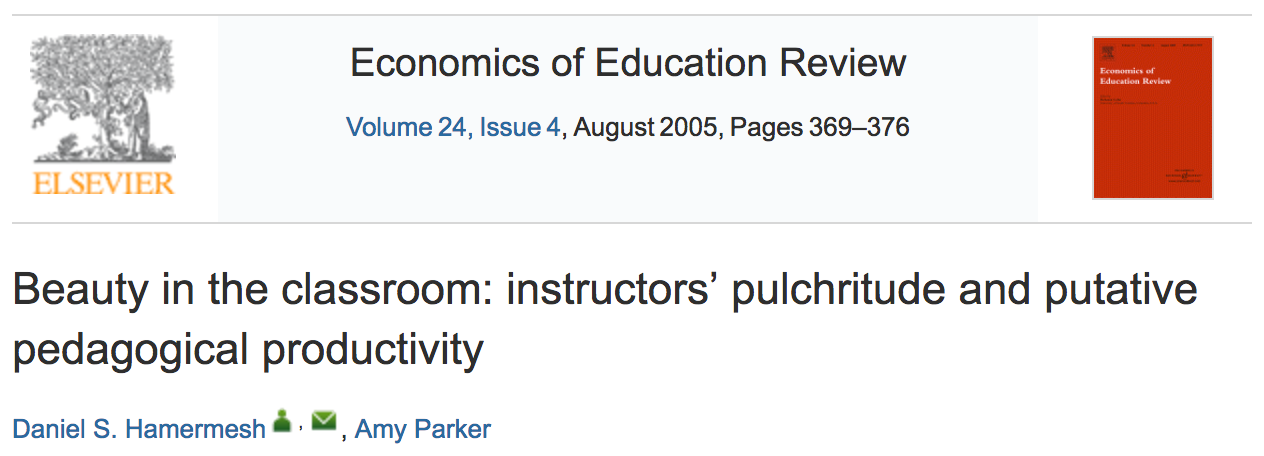
\includegraphics[width=\textwidth]{hamermesh}
    \end{frame}

    \begin{frame}{Hamermesh \& Parker (2005) data set}
      \begin{itemize}
        \item Student evaluations of $N=463$ instructors at UT Austin, 2000-2002
        \item For each instructor:
          \begin{itemize}
            \item \textbf{beauty}: average score from a six-student panel)
            \item \textbf{gender}: male or female
            \item \textbf{credits}: single- or multi-credit course
            \item \textbf{age}: age of instructor
            \item (and more...)
          \end{itemize}
      \end{itemize}
    \end{frame}

    

    \begin{frame}{Explore the data}
      \note{
        Before showing this, ask students how you might explore the impact \textCR
        of gender on evaluation scores. If someone suggests comparing the \textCR
        means, ask how you might graphically display it. \textCR
        After displaying the graph, elicit what we can conclude---the mean \textCR
        is higher for men, but the spread also looks larger.  Use this as \textCR
        an opportunity to quickly review variance/SD.
      }
\begin{knitrout}
\definecolor{shadecolor}{rgb}{0.969, 0.969, 0.969}
\input{/tmp/figures/unnamed-chunk-3-1.tex}

\end{knitrout}
    \end{frame}

    \begin{frame}{Explore the data}
      \note{
        Before showing this, ask students how you might explore the impact of \textCR
        single vs multi credit courses on evaluation scores. Ask students to \textCR
        speculate on the cause.
      }
\begin{knitrout}
\definecolor{shadecolor}{rgb}{0.969, 0.969, 0.969}
\input{/tmp/figures/unnamed-chunk-4-1.tex}

\end{knitrout}
    \end{frame}

    \begin{frame}{Explore the data}
      \note{
        Before showing this, ask students how you might explore the impact of \textCR
        beauty on evaluation scores, and ask students to predict the effect.
      }
\begin{knitrout}
\definecolor{shadecolor}{rgb}{0.969, 0.969, 0.969}
\input{/tmp/figures/unnamed-chunk-5-1.tex}

\end{knitrout}
    \end{frame}

    \begin{frame}{Explore the data}
      \note{
        Before showing this, ask students to predict the effect of age on \textCR
        evaluation scores.
      }
\begin{knitrout}
\definecolor{shadecolor}{rgb}{0.969, 0.969, 0.969}
\input{/tmp/figures/unnamed-chunk-6-1.tex}

\end{knitrout}
    \end{frame}

    \begin{frame}{Build the model}
      
      \begin{center}
        A regression model lets us create a model that incorporates all of these relationships to best predict evaluation scores:
        \[
          \widehat{\text{eval}} =
            4.13 +
            0.16 \cdot \text{beauty} -
            0.2 \cdot \text{female} +
            0.58 \cdot \text{credits} +
            0 \cdot \text{age}
        \]

        \pause

        We predict a 40-year-old female, with a beauty score of 2, teaching a multi-credit course would get an evaluation score of
        \[
          \widehat{\text{eval}} = 4.13 + 0.16 \cdot 2 - 0.2 \cdot 1 + 0.58 \cdot 0 = 4.18.
        \]

      \end{center}
    \end{frame}

    \begin{frame}{Evaluate the model}
      How could you evaluate the quality of this model?
    \end{frame}

    \begin{frame}{Can we do better?}
      \note{
        The pattern is different for men and women---beauty makes more of \textCR
        a difference for men. We probably will not have time to go into it\textCR
        any further; this is just to whet students' appetite for what is possible.
      }
      Do you see a difference between men (blue) and women (red)?

\begin{knitrout}
\definecolor{shadecolor}{rgb}{0.969, 0.969, 0.969}
\input{/tmp/figures/unnamed-chunk-8-1.tex}

\end{knitrout}
    \end{frame}

    \begin{frame}{Can we do better?}
      \note{
        The pattern is different for men and women---beauty makes more of \textCR
        a difference for men. We probably will not have time to go into it\textCR
        any further; this is just to whet students' appetite for what is possible.
      }
      Do you see a difference between men (blue) and women (red)?

\begin{knitrout}
\definecolor{shadecolor}{rgb}{0.969, 0.969, 0.969}
\input{/tmp/figures/unnamed-chunk-9-1.tex}

\end{knitrout}
    \end{frame}

    \begin{frame}{Five for the weekend}
      \begin{enumerate}
        \item Read the syllabus
        \item Install R and RStudio on your computer
        \item Make sure you can log in to Canvas
        \item Bring a laptop to class on Monday (and every day)
        \item Take the pretest (by January 31)
      \end{enumerate}
    \end{frame}


  \end{darkframes}

\end{document}
